\documentclass[fontsize=11, titlepage=true, parskip=half]{scrartcl}
\usepackage{geometry}			%Papierformat und Rand
\geometry{a4paper, left=2cm, right=2cm, top=2cm, bottom=2cm}
\usepackage[utf8]{inputenc}
\usepackage[ngerman]{babel}
\usepackage{amsmath}
\usepackage{amssymb}
\usepackage{pdfsync}
\usepackage{pdflscape}			%landscape Umgebung für Querformatanzeige
\usepackage{siunitx}			%schöne SI Einheiten
\usepackage{graphicx}
%\usepackage{abstract}			%??
%\usepackage{microtype}		%saubere Umbrüche bei mehrspaltigen Docs
\usepackage{booktabs}			%??
\usepackage[hyphens]{url}
\usepackage{eurosym}			%schönes Euro Symbol
%\usepackage{dblfloatfix}		%float bottom twocolumn
\usepackage[hidelinks]{hyperref}	% Paket: ltxcmds kann Links stylen
\usepackage[automark]{scrlayer-scrpage} 	%Kopf und Fußzeile bearbeiten Paket: koma-script
\chead*{\pagemark} %Seitenzahl mittig in Kopfzeile
\cfoot[]{} %Voreinstellung für Seitenzahl löschen
\usepackage{color}				%eigene Farben definieren (für Code-Highlighting)
\usepackage[comma]{natbib}
\usepackage[onehalfspacing]{setspace} %Zeilenabstand 1.5
\newcommand{\csharp}{{\settoheight{\dimen0}{C}C\kern-.05em \resizebox{!}{\dimen0}{\raisebox{\depth}{\#}}}} %schönes C#

\usepackage{multirow}
\usepackage{tabularx} %für feste Tabellenbreite und Umbrüche in Spalten
\usepackage{ragged2e} %"'"'
\newcolumntype{L}[1]{>{\raggedright\arraybackslash}p{#1}}
\newcolumntype{C}[1]{>{\centering\arraybackslash}p{#1}}
\newcolumntype{R}[1]{>{\raggedleft\arraybackslash}p{#1}}
\newcolumntype{J}[1]{>{\justifying\arraybackslash}p{#1}}


%Farben für C#
\definecolor{bluekeywords}{rgb}{0,0,1}
\definecolor{greencomments}{rgb}{0,0.5,0}
\definecolor{redstrings}{rgb}{0.64,0.08,0.08}
\definecolor{xmlcomments}{rgb}{0.5,0.5,0.5}
\definecolor{types}{rgb}{0.17,0.57,0.68}

%Farben für HTML


%Listings für Code
\usepackage{listings}
\lstset{frame=lines, % Oberhalb und unterhalb des Listings ist eine Linie
showstringspaces=false,
basicstyle=\ttfamily\small,
showspaces=false,
showtabs=false,
breaklines=true,
breakatwhitespace=true,
escapeinside={(*@}{@*)},
}

\lstdefinestyle{CSharp}{language=[Sharp]C,
captionpos=b,
%numbers=left, %Nummerierung
%numberstyle=\tiny, % kleine Zeilennummern
commentstyle=\color{greencomments},
morekeywords={partial, var, value, get, set},
keywordstyle=\color{bluekeywords},
stringstyle=\color{redstrings},
}

\lstdefinestyle{HTML}{language=HTML,
% sensitive=true,
% classoffset=0,	
% stringstyle=[0]\color{bluekeywords},
% keywordstyle=[0]\color{redstrings},
% classoffset=1,
% morekeywords={
% %Angular
% [(ngModel)], (change), *ngIf,
% },
% keywordstyle=[1]\color{red},
}

\AfterTOCHead{
\singlespacing
\thispagestyle{empty}
}



% \includeonly{
% Titelblatt2,
% Abstract,
% Einleitung,
% Problembeschreibung,
% Grundlagen,
% Analyse_des_Problems,
% Lösung,
% Zusammenfassung_und_Diskussion,
% Fazit_und_Ausblick,
% }

\begin{document}
\pagenumbering{roman}
\titlehead{
{\Large Hochschule Rhein Waal}\\
Fakultät für Kommunikation und Umwelt\\
Friedrich-Heinrich-Allee 25\\
47475 Kamp-Lintfort
}

\subject{
Abschlussbericht\\
\normalfont
im Modul Wissenschaftliches Arbeiten\\
}

\title{Deepfake}

\subtitle{Kann die aufkommende Gefahr von Audio Deepfakes mit technischen Hilfsmitteln abgewendet werden?}
\author{
Dario Becker
\thanks{
 Matr.-Nr.: 28492\\
E-Mail: dario.becker@hsrw.org}
\and Timo Hungenberg
\thanks{
Matr.-Nr.: 28501\\
E-Mail: timo.hungenberg@hsrw.org}
}

\date{\today}

% \publishers{
% Betreut durch\\
% Tobias Scharlewsky
% \thanks{
% Telefon: +49(203)41752945\\
% E-Mail: tobias.scharlewsky@polizei.nrw.de}\\
% Prof. Dr. Thomas Richter}

\maketitle


\tableofcontents

\cleardoubleoddpage
\pagenumbering{arabic}
%\KOMAoption{parskip}{half}

\section{Einleitung}
% Hier Deepfakes im allgemeinen Vorstellen: Welche Arten gibt es und wie werden die verbreitet?
% Aktuelles Thema als Einführung in unsere konkrete Problematik: Von Deepfake allgemein zu Teilaspekt führen den wir besprechen.
% Enden mit Forschungsfrage bzw. Ziel des Artikel: Was wollen wir zeigen, worauf wollen wir hinaus?
In der heutigen Zeit nimmt das Aufkommen und die Verbreitung von Falschmeldung zu \citep[][]{Hancock2021}.
Besonderen mehren sich die mit Hilfe von künstlicher Intelligenz erschaffene manipulierte Falschmeldungen, sogenannte Deepfakes \citep[][]{Shahzad2022}.
Der Begriff des Deepfake entsteht aus ``Deeplearning'', eine auf künstlicher Intelligenz basierter Methode des maschinellen Lernens, und ``Fake'' welcher mit Hilfe dieses ``Deeplearnings'' erstellt wird und den Menschen täuschen soll \citep[][]{Mueller2022}.
Innerhalb der Deepfakes werden z.B. Gesichter in eine Bild- oder Videodatei realistisch geschnitten, um diese Personen beliebige Worte sagen zu lassen.
So zeigt ein aktuelles Beispiel, wie Olaf Scholz eine angebliche Rede hält in der er über russische Gaslieferungen spricht \citep[][]{Klasen2022}.
Über Twitter wird die Reaktion Putins auf diese Rede von einer russischen Nachrichtenagentur geteilt \citep[Vgl.][]{Klasen2022}.
Gerade über die Kanäle der sozialen Medien wie Twitter oder Facebook, lassen sich diese Falschmeldungen heutzutage schnell und gezielt verbreiten (siehe Putin-Scholz Beispiel).
\par
Eine weitere Form des Deepfakes ist die Manipulation von Audiodateien (Audio Deepfakes, AD).
Diese Art Deepfake oftmals von Betrügern genutzt wird, um potentielle Opfer am Telefon oder in Interviews zu täuschen, also in Echtzeit \citep[][]{Mueller2022}.
Wie bereits einige Fälle gezeigt haben \citep[Vgl.][]{Stupp2019}, nimmt die zeitliche Komponente bei der Erkennung dabei eine besondere Rolle ein.
Denn ist der Deepfake einmal geteilt und in den Köpfen der Menschen, lassen sich Falschmeldungen nur schwierig korrigieren \citep[][]{Hancock2021}.
Dabei ist die nachträgliche Abwendung der Gefahr von Echtzeit-, also oftmals AD, dabei weitaus schwieriger als auf sozialen Medien Geteilten Video- oder Bildmaterialien \citep[][]{Shahzad2022}.
\par
% Um Deepfakes als soche zu Erkennung, werden in der Literatur einige Merkmale wie z.B. die Asynchronität von Stimme und Lippenbewegung genannt \citep[][]{Appel2022}.
% Auch das zu häufige Blinzeln, Kopfhaltung oder Falschstellungen von Zähnen, können ein Indiz auf einen Deepfake sein \citep[][]{Shahzad2022}.
Da die menschliche Wahrnehmung zur Erkennung eines Deepfakes allerdings limitiert ist, empfehlen Wissenschaftler den Einsatz von technischen Hilfmitteln \citep[][]{Mueller2022}.
Zwar wird sich für Maßnahmen ausgesprochen um gegen Deepfakes zu sensibilisieren, aber das wird zukünftig nicht reichen da die Technologie zur Erstellung solcher Deepfakes immer besser wird \citep[][]{Amezaga2022}.
% Daher ist es unbedingt notwendig, dass die Erkennung mit technischen Hilfsmitteln weiterentwickelt werden muss.
% Es gibt einige technische Lösungen zur Erkennung von Audio-Deepfakes, die ähnlich wie die Erstellung von Deepfakes auf künstlicher Intelligenz basieren, welche aber den zeitlichen Faktor nicht berücksichtigen.
\par
In dieser Arbeit wird aufgezeigt, welche Gefahrenpotentiale AD beinhalten, wie die menschliche Wahrnehmung zu solchen Fakes ist und wie die Technik dabei helfen kann diese in Echtzeit zu entlarven.
Dabei werden verschiedene Methoden zur Erstellung und Erkennung solcher Fakes analysiert und diskutiert.
Vor allem werden die beiden Methoden Text-to-Speech und Voice Conversion, welche aktuell überwiegend zur Erzeugung von AD genutzt werden, genauer untersucht.
Die Frage, ob und in welchem Grad AD mit Hilfe aktueller technischer Lösungen in Echtzeit erkennbar sind, wird in mehreren Herausforderungen unterteilt, analysiert und beantwortet.
Dabei ist das Ziel dieser Fragestellung, welche Art von AD mit welchen Ansätzen der technischen Erkennung in welcher Zeit zu erkennen sind und wie die davon abgeleitete zukünftige Behandlung solcher Fakes zu gestalten ist. 

\section{Gefahrenanalyse und Einfluss von Deepfakes auf den Menschen}
% Gesellschaftliche Betrachtung der Thematik.
% 2-3 Sätze die erklären, was im Kapitel passiert.
In diesem Kapitel werden die Angriffspunkte von Deepfakes und den damit verbundenen Gefahren für die Gesellschaft beschrieben.
Anhand einiger Beispiele wird aufgezeigt, welchen Einfluss Deepfakes haben, um beim Menschen durch gezielte Manipulation Schaden anzurichten.
Weiterhin werden Möglichkeiten zur schnelleren Erkennung solcher Manipulationen diskutiert.
\subsection{Gefahrenpotential allgemein}\label{Gefahrenpotential}
% Hier zunächst allgemeine Gefahrenpotentiale von gezielter Fehlinformation definieren.
Das Konzept der Falschinformation, in der heutigen Zeit oft unter dem Begriff ``Fake News'' genannt, ist eine Methode die bereits seit mehr als 125 Jahren eingesetzt wird um Menschen gezielt zu manipulieren.
Gerade im Zeitalter der sozialen Medien, in denen sich Menschen öfter dieser Meldungen bedienen als konventioneller Nachrichten, wächst die Bedrohung durch Falschinformation täglich (\cite{Lee2019}).
Eine große Gefahr die dabei von Deepfakes ausgeht, ist dass jeder die Möglichkeit hat, diese mit kostenfreier Software zu erstellen (\cite{Appel2022}).
Das gefährliche dabei ist die millionenfache Verbreitung innerhalb Sekunden um die ganze Welt, in der Jeder Ziel eines solchen Angriffs sein kann (\cite{Shahzad2022}).
\par
Dabei nennen Appel und Prietzl (\cite{Appel2022}) Angriffsziele von privaten Personen, über Prominente Personen bis hin zu ganzen Staaten.
Besonders letzteres ist ein immer häufiger gewähltes Ziel, gerade bei politschen Wahlen oder Zwischenstaatlichen Beziehungen.
So kursierte im März 2022 in sozialen Medien ein Deepfake-Video des Ukrainischen Präsidenten Volodymyr Zelenskyy, in dem er im Rahmen des Russisch-ukrainischen Krieges die Kapitulation seiner Soldaten forderte.
Einmal durch die Kanäle sozialer Medien verbreitet, lassen sich diese Falschmeldungen schwierig Löschen oder Richtigstellen und wenn doch, dann ist der Schaden bereits angerichtet.
Soziale Netzwerke oder Messenger wie Facebook, WhatsApp oder Telegram sind dabei besonders kritisch zu betrachten, da sie die Verbreitung von ungeprüften Inhalten jeglicher Art ermöglichen (Vgl. \cite{Appel2022}).
\par
Deepfakes erweitern und verschlimmern also das bereits bekannte Phänomen der ``Fake News'', indem sie sich der gleichen Kanäle bedienen, die Inhalte allerdings noch deutlich realistischer und glaubhafter darstellen (\cite{Appel2022}).
Gerade das hohe Level von Faktoren wie Verbreitungsgeschwindigkeit, Realismus und Personalisierung machen Deepfakes zu einer immer weiter wachsenden Gefahr für die Gesellschaft.
Was den Menschen dabei so angreifbar macht, ist die Tatsache, dass vermeintlich selbst wahrgenommen Inhalte wie Videos und Fotos, einen stärkeren Eindruck hinterlassen als niedergschriebener Text.
Besonders wenn es sich dabei um vertraute Personen und deren Auftreten oder Stimme handelt (\cite{Kietzmann2020})
\newpage

\subsection{Gefahrenanalyse am Beispiel aktueller Fälle}\label{GefahrenAktuelleFaelle}
% Gefahrenpotentiale an Beispielen konkretisieren: \textbf{Was} wurde gemacht um \textbf{was} zu erreichen?
% Hier Fokus auf Echtzeitproblematik legen? Oder folgt das aus dem nächsten Unterkapitel?
Folgend werden einige aus dem unter Abschnitt \ref{Gefahrenpotential} beschriebenen Gefahren anhand konkreter Realfällen diskutiert.
Bei diesen Fällen handelt es sich hauptsächlich um Betrugsfälle, die mit Hilfe von Deepfakes durchgeführt wurden.
\par
Einer dieser Fälle, der im Zusammenhang mit Deepfake-Betrug genannt wird, ist die Erbeutung von 220.000\euro{} durch Verwendung eines Audio-Deepfakes.
In diesem Fall stellten Betrüger die Stimme eines CEO am Telefon nach und baten seinen angeblichen Mitarbeiter, den genannten Betrag auf ein Konto zu überweisen (CITE ONLINE QUELLE?!).
Der angerufene Mann berichtete nachträglich an die Ermittlungsbeamten, dass er den deutschen Akzent und die Melodie der Stimme seines CEO's erkannte, und somit keinen Verdacht schöpfte dass es sich bei diesem Anrufer um einen Betrüger handelte.
Die Ermittlungen gingen davon aus, dass eine kommerzielle Software zur Erstellung des Deepfakes verwendet wurde.
Dieses Beispiel verdeutlicht, dass jeder mit entsprechender freizugänglicher Software im Stande ist, so einen Betrug mit Hilfe eines Audio-Deepfakes durchzuführen. (CITE ONLINE QUELLE?!).
\par
Eine weitere Betrugsmasche, vor der das FBI offiziell warnte, sind Betrugsfälle in denen sich mit durch Video Deepfake veränderter Stimme für sensible Jobs beworben wird.
Während dieser Jobinterviews, die meist auf Jobs mit Heimarbeit in Softwareunternehmen mit großen Datenmengen abzielen, benutzen Betrüger die Stimme einer anderen Person.
Das FBI betonte hierbei aber, dass die Synchronisation zwischen Lippenbewegung und Sprache nicht komplett übereinstimmte.
Somit gibt es Anhaltspunkte zur Vorbeugung und Erkennung solcher Betrüge in Form von Jobinterviews, indem Mitarbeiter von Unternehmen geschult werden um unter anderem auf solche Merkmale verschärft zu achten (CITE QUELLE FBI).
\par
Zur Veranschaulichung der potentiellen politschen Manipulation unter der Verwendung von Deepfakes, ist die Rede der amerikanischen Politikerin Nancy Pelosi aus dem Jahr 2019 zu nennen (ZITIER https://perma.cc/A26H-4PF3?type=image).
In dieser Rede wurde das Videomaterial so manipuliert, dass es so scheint als ob sie stotterte und undeutlich rede.
Das manipulierte Video wurde von dem zu dieser Zeit amerikanischen Staatspräsidenten und Anhänger der Gegnerpartei von Nancy Pelosi, Donald Trump, über Twitter verbreitet.
Er teilte es mit den Worten ``Pelosi stammers through news conference'', also mit der gezielten Absicht sie mit Hilfe dieses Videos zu diffamieren (ZITIER https://perma.cc/A26H-4PF3?type=image).
\par
Dieses Video zeigt die Gefahr der schnellen Verbreitung von ungeprüften Inhalten durch soziale Medien, die unter Abschnitt \ref{Gefahrenpotential} genannt wurde.
Über Facebook wurde dieses Video über 2.5 Millionen mal angeschaut, Facebook selbst lies dieses Video auf der Plattform bestehen versprach aber die Verbreitung einzugrenzen.
Youtube hingegen löschte dieses Video, da es sich um falsche Inhalte handelte.
Dieses unterschiedliche Behandeln von Falschinformation verschiedener sozialer Medien zeigt die Schwierigkeit des Konsums von Informationen über diese Plattformen.
Es bleibt daher ein beliebtes Mittel zur Verbreitung solcher Inhalte, eben aufgrund der freien Verbreitung, Geschwindigkeit und umständlicher Löschung dieser (\cite{Appel2022}).
\par
Die hier beschriebenen Betrugsfälle veranschaulichen, dass wie unter Abschnitt \ref{Gefahrenpotential} beschrieben, mit einfachsten Mitteln großer Schaden angerichtet werden kann.
Besonders die von Kietzmann (\cite{Kietzmann2020}) beschriebene Vertrautheit von Inhalten wie z.B. die Stimme im Zusammenspiel mit Gestik und Mimik, ließ bei den erwähnten Beispielen keinen Zweifel an der Echtheit.
So reichte es bei dem Telefonbetrug, dass der deutsche Akzent und die Melodie der Stimme vermeintlich übereinstimmte, keinen Verdacht zu schöpfen.
Darüberhinaus zeigen die genannten Beispiele, dass die Echtzeit und damit die nahezu nicht vorhandene Zeit zur Erkennung eine entscheidene Rolle spielt.
Einmal verbreitet lässt sich der Schaden nur erschwert beheben oder die Inhalte schwierig Löschen oder Richtigstellen (\cite{Shahzad2022}).
Dabei betonte Shahzad (\cite{Shahzad2022}) einmal mehr, zukünftig effektive Methoden zur Erkennung in Echtzeit zu entwickeln, da diese den Großteil der Bedrohung darstellen.
Ein weiteres Gefahrenpotential bleibt der einfache Zugang zur Erstellung solcher Deepfakes.
Mit den richtigen Zugängen zu Verbreitungskanälen und anzusprechenden Opfern, ist es jedem Menschen möglich das Mittel der Manipulation durch Deepfakes zum Betrug einzusetzen (\cite{Appel2022}).




\subsection{Gefahrenanalyse/Studien zur menschlichen Wahrnehmung}
% Analyse von durchgeführten Studien: Inwieweit ist der Mensch anfällig für Deepfakes?
% Welche Konsequenz ergibt sich daraus? (Anforderungen an Informationen, Detektion von DF, etc.)
Folgend werden Ergebnisse mehrerer Studien betrachtet, um den Einfluss und die damit verbundenen Gefahren von Deepfakes auf den Menschen zu betrachten.
Die menschliche Wahrnehmung von Deepfakes sowie Folgen der Manipulation spielen sind dabei Hauptfaktoren.
\par
Um zu untersuchen, ob und mit welchem Umfang Deepfakes im politschen Rahmen Wähler beeinflussbar sind, manipulierten Wissenschaftler der Amsterdamer Universität Videomaterial eines holländischen Politikers \citep[Vgl.][]{Dobber2020}.
In diesem dreizehn sekündigen Video beinhalten die letzten fünf Sekunden manipuliertes Material in dem der folgene Satz fällt ``But, as Christ would say: don’t crucify me for it''.
Sie wählten diesen Satz, da dieser Politker einer konservativen christlichen Partei angehörte und somit die potentielle Wahlzielgruppe anspricht.
Dabei nutzte diese Studie politisches Microtargeting, ein von Parteien zur Beeinflussung von Wählern häufig gewähltes Mittel, indem es auf die religiöse Einstellung abzielte \citep[Vgl.][]{Papakyriakopoulos2017}.
\par
An dieser Studie nahmen 277 Menschen teil, von denen 144 Teilnehmer das manipulierte Video und 133 das Originalvideo sahen.
Schlüsselfaktoren zur Einteilung und Unterscheidung waren unter anderem die Religiösität und die politische Einstellung.
Als Ergebnis betrachtete die Studie die Einstellung der Teilnehmer gegenüber dem Politker und seiner Partei.
Gläubige Menschen, die das manipulierte Videon sahen, hatten eine schlechtere Einstellung zum Politker als vorher.
Dabei galt diese schlechtere Einstellung eher dem Politiker direkt, als seiner angehörigen Partei.
Von den 144 Teilnehmern, die das manipulierte Video sahen, erkannten nur 12 den Fake.
Zukünftige Erstellung von realistischeren Deepfakes könnte dies aber ändern, Potential zur Manipulation durch Deepfakes sei gegeben.
Durch die Verwendung von Deepfakes lassen sich Menschen leichter manipulieren als durch klassische ``Fake News'' \citep[][]{Dobber2020}.
Weiterhin kam die Studie zum Fazit, dass sich aufgrund der geringen Anzahl von 12 Leuten die den Fake erkannten, die Sensibiliserung der Gesellschaft für solche Deppfakes verbessern sollte.
Diese Studie zeigt die Gefahr der Fähigkeit, eine bestimmte politische oder demographische Gruppe anzusprechen.
Es kann also gezielt Microtargetting über soziale Medien betrieben werden \citep[Vgl.][]{Hancock2021}.
\newpage
Zur Analyse, ob und wie der Mensch manipulierte Audiodateien erkennt, erschufen sie ein rundenbasiertes Spiel \citep[][]{Mueller2022}.
In Jeder Runde, hörten die Teilnehmer eine Audio und mussten wählen ob diese echt oder gefaked ist.
Dazu hörten die 410 Teilnehmer insgesamt 13229 Audiodateien, wobei nur gezählt wurde wenn mindestens 10 Runden absolviert waren.
\par
\begin{figure}[h]
 \centering
 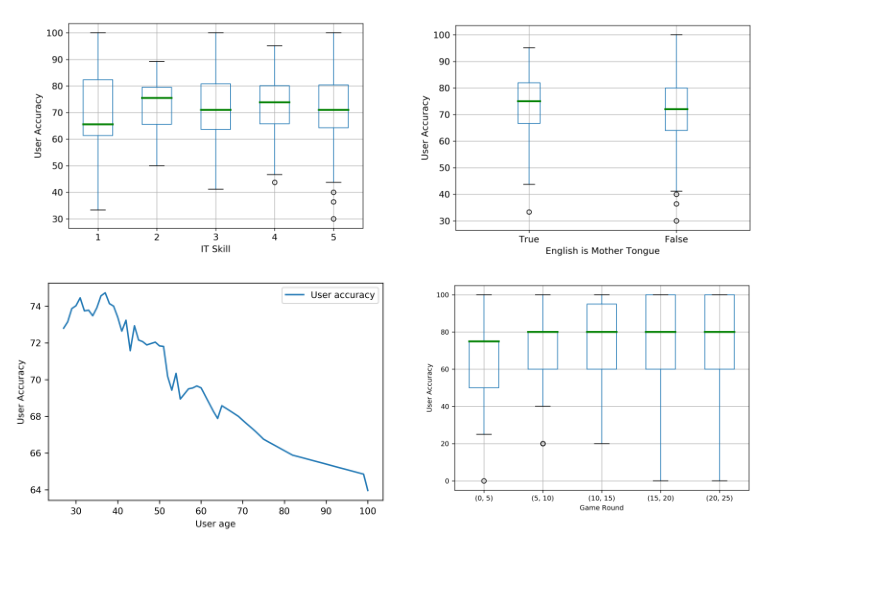
\includegraphics[width=\textwidth]{Assets/ResultsHumanDetectionDeepFake.png}
 \caption{Menschliche Wahrnehmung von Audio Deepfakes \citep[][]{Mueller2022}.}
 \label{fig:ResultsDetectionDeepfake}
\end{figure}
Die Teilnehmer wurden an Faktoren wie Alter, IT-Erfahrungen und Muttersprachler (die Studie wurde in englischer Sprache durchgeführt) kategorisiert.
Unter Abbildung \ref{fig:ResultsDetectionDeepfake} sind die Ergebnisse zu erkennen, in denen die Genauigkeit der Erkennung dem jeweiligen Personenkreis gegenüber gestellt ist.
Muttersprachler haben Vorteile bei der Erkennung von Fakes gegenüber Fremdsprachlern.
Weiterhin sei die IT-Kenntniss irrelevant, mit zunehmendem Alter verschlechterte sich die Genauigkeit. 
In den Ersten Runden nimmt die Genauigkeit bei der Erkennung zu, stagniert dann aber nach etwa 20 Runden.
Schaffung der Förderung von zukünftigen Gegenmaßnahmen werden benötigt, da sich die Qualität der Audio-Deepfakes erhöht, die menschlichen Fähigkeiten zur Erkennung allerdings stagnieren \citep[][]{Mueller2022}.
\par
Zur Untersuchung, welchen sozialen Einfluss Deepfakes auf den Menschen haben, verbindet Hancock das Verhalten des Menschen auf generelle Falschinformationen mit der Täuschung von Deepfakes.
Menschen sind, so Hancock, nicht gut darin Falschinformationen als solche zu erkennen.
Es wird dazu geneigt, eher an das zu Glauben was gesehen wird.
Das gefährliche an Deepfakes ist die manipulierte Kombination von z.B. Stimme, Mimik und Gestik.
Während einer dieser Faktoren schon schwierig als Falschinformation zu entlarven ist, verstärkt diese Kombination durch Vertrautheit der Wahrnehmung die Glaubhaftigkeit des Fakes \citep[Vgl.][]{Hancock2021}.
Durch Sensibilisierung lassen sich die Effekte schmälern, so vergleich Hancock es mit der Existenz von Spammails, deren Gefahr durch allgemeine Bekanntheit innerhalb der Gesellschaft verringert ist.







% Analyse von durchgeführten Studien: Inwieweit ist der Mensch anfällig für Deepfakes?
% Welche Konsequenz ergibt sich daraus? (Anforderungen an Informationen, Detektion von DF, etc.)
\section{Technische Erkennung von Audio Deepfakes}
% Analyse der verfügbaren Detektionsalgorithmen auf Effektivität und Effizienz im Hinblick auf Echtzeitproblematik
% 2-3 Sätze die erklären, was im Kapitel passiert.
Dieser Abschnitt befasst sich mit verschiedenen methodischen Ansätzen zur Erkennung von AD, wobei der Fokus auf der Erkennung von Deepfakes in (nahezu) Echtzeit liegt.
Wie aus den vorangegangenen Abschnitten deutlich wird, sind gerade die schnelle Verbreitung und die damit verbundene geringe Reaktionszeit die größten Probleme bei der Bekämpfung von Deepfakes.
Speziell die Verwendung von AD als Grundlage für möglichen Telefonbetrug ist hier besonders kritisch zu betrachten, da im Gegensatz zu beispielsweise dem Veröffentlichen von Videomaterial auf Social Media keine (zeitaufwendige) technische Überprüfung der Inhalte möglich ist.
Diese potentielle Gefahr soll im Folgenden als Referenz für die Bewertung der aktuell verfügbaren Detektionsalgorithmen dienen.
\subsection{Methodische Ansätze}
% Hier verfügbare Methoden kategorisieren und allgemein vorstellen.
% Welche Ansätze gibt es?
% Welche Voraussetzungen und Anforderungen haben die (Ressourcen, Quelle)?
In den letzten Jahren ist eine Häufung an Übersichtsartikeln über Detektionsalgorithmen für AD in der Fachliteratur zu beobachten \citep[][]{Masood2022,Almutairi2022,Khanjani2021}.
Tatsächlich sind dies die ersten Übersichtsartikel die konkret zu diesem Thema erschienen sind, der älteste wurde 2021 veröffentlicht \citep[][]{Khanjani2021}.
Das zeigt wie frisch und hochaktuell die wissenschaftliche Auseinandersetzung mit der Thematik AD ist.
Außerdem fällt auf, dass viele unterschiedliche Ansätze von verschiedenen Forschungsgruppen zu finden sind.
Hier scheint sich eine Community zu formen, die sich einen ersten Überblick über die unterschiedlichen Ausprägungen ihrer Forschung verschaffen will.

Diesen Überblick wollen wir nutzen, um zu untersuchen inwieweit die aktuell erforschten Detektionsalgorithmen bei der zeitkritischen Bekämpfung von AD unterstützen können.
Dazu werden zunächst die grundsätzlichen Methoden zur Erzeugung und Detektion von AD vorgestellt, da diese unweigerlich miteinander verbunden sind.
Anschließend werden diese hinsichtlich der Voraussetzungen und Anforderungen an benötigte Ressourcen sowie die Audioquelle selbst analysiert.
Dabei stellt sich stets die Frage, ob die Technologie bereits jetzt oder eventuell in naher Zukunft prinzipiell einen Telefonbetrug schnell genug aufdecken kann, um diesen verhindern zu können.

\subsubsection{Erzeugung von Audio Deepfakes}
Zur Erzeugung von künstlichen Audiospuren werden aktuell vor allem zwei Methoden verwendet.
Der größte Unterschied ist dabei das Ausgangsmedium.
So findet bei Text-to-Speech (TTS) eine Konvertierung von Text in Sprache statt, während es bei der Voice Conversion (VC) darum geht, ein bestehendes Audiofile zu manipulieren.
Im Folgenden werden diese beiden Arten der Erzeugung von künstlichen Audiospuren vorgestellt und einige Vor- und Nachteile sowie daraus resultierende Einsatzgebiete zusammengefasst.
\clearpage

\textbf{Text-to-speech}\\
%Bei der Erzeugung von Audio Deepfakes ist dabei immer das Ziel, eine Audiospur zu erzeugen, die der einer realen Zielperson möglichst ähnlich ist.
Text-to-speech wurde entwickelt, um Mensch-Computer-Interaktionen zu vereinfachen.
Beispielsweise können so Texte durch Screenreader oder Navigationsanweisungen vorgelesen werden.
Der grund"-sätzliche Prozess ist in Abbildung~\ref{fig:tts} \citep[][]{Masood2022} dargestellt.

\begin{figure}[htp]
\begin{center}
  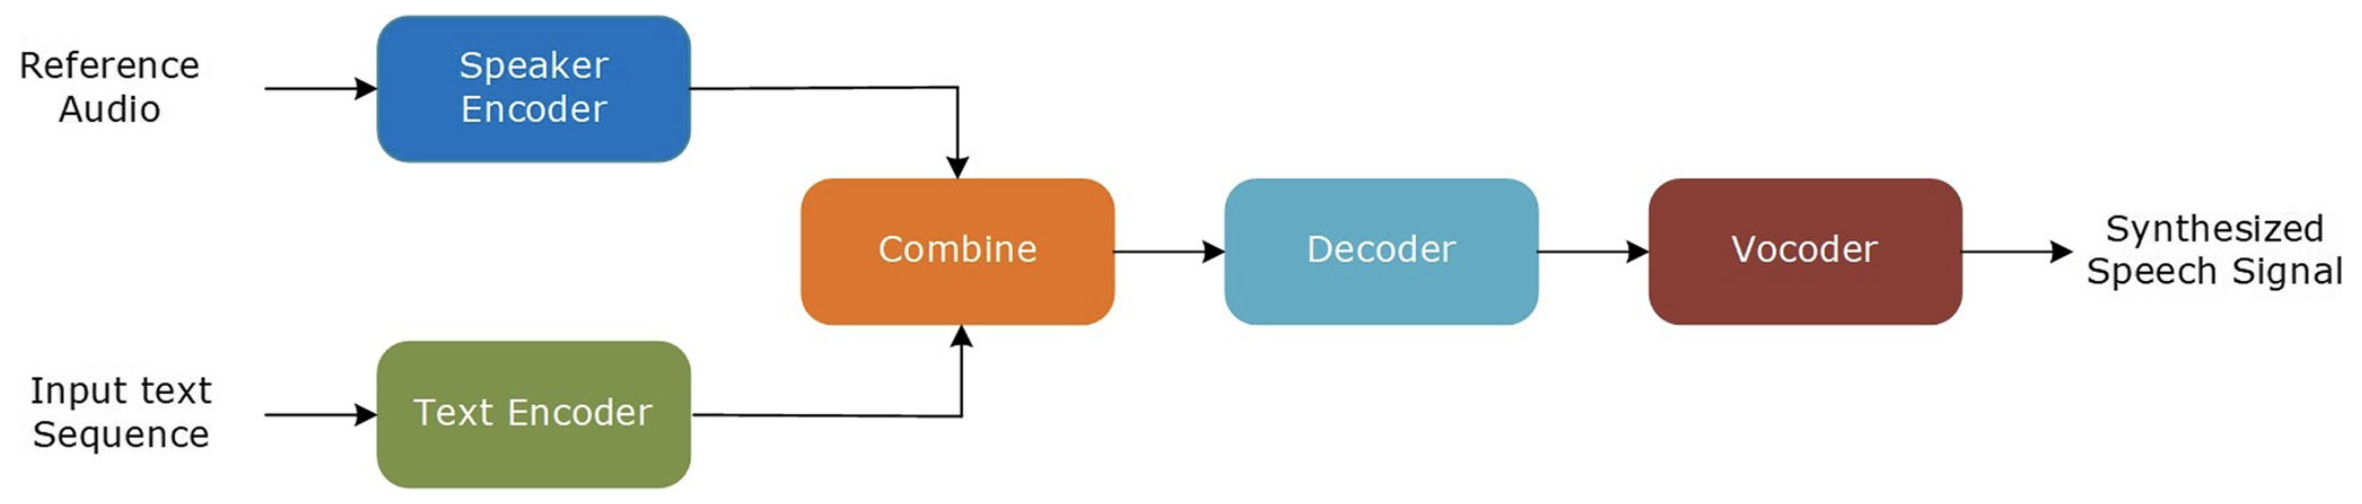
\includegraphics[width=0.95\textwidth]{assets/TTS.png}
  \caption[labelInTOC]{Workflow Diagramm der aktuellen TTS Systeme \citep[][]{Masood2022}}
  \label{fig:tts}
\end{center}
\end{figure}

Zunächst wird ein TTS Modell mithilfe von Audioaufnahmen sowie den dazugehörigen Transkripten auf eine Stimme trainiert.
Anschließend können Texte entgegengenommen, in zuvor gelernte Formen gebracht und so die Parameter für den letzten Schritt berechnet werden.
Mit diesen Parametern wird mittels Vocoder ein Audiosignal erzeugt, das dem gewünschten Text in einer möglichst menschenähnlichen Stimme entspricht.
Einige Beispiele für derartige Deeplearning Modelle sind WaveNet (2016), Tacotron2 (2018) und DeepVoice3 (2018) \citep[vgl.][]{Almutairi2022}.

Neueste Entwicklungen zeigen, dass dieser Prozess auch in Echtzeit möglich ist, wobei von Voice Cloning gesprochen wird.
Hierbei liegt der Fokus darauf, bestimmte Stimmfeatures zu erhalten wodurch nicht nur menschenähnliche Stimmen sondern gezielt Personen nachgeahmt werden können.
Diese Technologie ist frei zugängig, beispielsweise über Anwendungen wie Overdub oder VoiceApp und ermöglicht die Erstellung von AD \citep[][]{Masood2022}.

\textbf{Voice Conversion}\\
Eine andere Möglichkeit künstliche Sprachdateien zu erzeugen ist Voice Conversion.
Im Gegensatz zu TTS liegt als Eingabe eine Audiodatei vor, wobei die Stimme durch verschiedene Methoden so moduliert wird, dass die Ausgabe einer anderen Person zugeordnet werden kann.
Diese Modulierung basiert auf verschiedenen akustischen Features wie dem Stimmklang, der Betonung, Tempo und Sprechpausen.
Dementsprechend groß sind die Datenmengen, die benötigt werden um realistische Stimmen zu erzeugen.
Allerdings lassen sich so sehr gute Imitate erzeugen, zum Teil sogar in einer anderen Sprache, wenn die Qualität der zum Anlernen verwendeten Audiodaten entsprechen gut ist \citep[][]{Masood2022}.

Hier werden ähnlich wie bei TTS Vocoder verwendet, aber auch Neuronale Netze und Machine Learning mit speziellen Algorithmen zur Manipulation von multimedialen Inhalten.

Beide Technologien, sowohl TTS als auch VC, eignen sich prinzipiell für die Erzeugung von AD in Echtzeit beziehungsweise zur Verwendung in oben genannten Szenarien.
Voraussetzung ist jeweils, dass genug Material der Zielperson vorhanden ist, um die Modelle anzulernen.
\clearpage

\subsubsection{Audio Deepfake Detection}
Die zuvor vorgestellten Methoden zur künstlichen Stimmsynthese werden nicht nur für die Verbesserung von Mensch-Computer-Interaktionen verwendet, sondern auch zur Erzeugung von AD mit zum Teil kriminellen Absichten.
Um dem entgegenzuwirken wird intensiv an Algorithmen zur Erkennung von AD geforscht.

Grundsätzlich können die verfügbaren Methoden darin unterschieden werden, ob die zur Identifizierung von synthetischen Audiospuren verwendeten Features manuell oder per Deeplearning spezifiziert werden.
Andere Quellen sprechen auch von feature-based approach oder image-based approach \citep[][]{Khochare2021}.
Bis auf wenige Ausnahmen ist allen Methoden gemein, dass sie auf die Detektion bestimmter Generationsmechanismen (TTS oder VC) spezialisiert sind.
Dabei werden sie auf definierte Sammlungen von synthetisch erzeugten Audiodateien mit bekannten Erzeugungsmechanismen angelernt um anschließend Proben mit ähnlichen Features identifizieren zu können.

Beim feature-based approach werden die einzelnen Audiodateien manuell auf verschiedene spektrale Features untersucht und in einen entsprechenden Datensatz umgewandelt.
Dieser Datensatz wird mit einem Machine Learning Algorithmus verarbeitet um dem Algorithmus beizubringen, welche Features in den später zu untersuchenden Proben relevant sind.
Beim image-based approach wird das Audiosignal mittels Fast Fourier Transformation von der Zeit- in die Frequenzebene umgewandelt und anschließend die Amplitude in Dezibel konvertiert um ein Melspectrogram zu erhalten.
Mit verschiedenen Deep Learning Methoden werden anschließend die relevanten Features berechnet.

Für beide Varianten sind große Datenmengen, bestehend aus vielen oder langen Sequenzen, zum Anlernen erforderlich.
In der Literatur werden einige Datensätze genannt, mit denen Detektionsalgorithmen angelernt, aber auch getestet werden können.
So gibt es einen sehr großen open source Datensatz von Mozilla \citep[][]{Ardila2019}, mittlwerweile vier Datensätze aus den Jahren 2015, 2017, 2019 und 2021 von der ASVspoof Challenge\footnote{Automatic Speaker Verification Spoofing And Countermeasures Challenge, bei der es darum geht aktuelle Herausforderungen in der Erkennung von Audio Deepfakes zu bewältigen um die Sicherheit von ASV Systemen zu erhöhen\citep[][]{Yamagishi2021}} sowie weitere öffentlich zugängige Datensätze wie den fake-or-real (FOR) Datensatz \citep[][]{Reimao2019}. 
Dabei geht der Trend dahin, nicht mehr nur die grundsätzlichen Fähigkeiten von Detektionsalgorithmen zur Überprüfung von (Labor)Proben zu beweisen, sondern es werden vermehrt Audioproben erzeugt und getestet, die einen realen Angriff mit Fake Audio simulieren sollen.
Der FOR sowie der aktuellste Datensatz der ASVspoof Challenge enthalten Proben, die einen Angriff per Telefon oder Sprachnachricht simulieren sollen \citep[][]{Masood2022}.

Sind die Detektionsalgorithmen einmal angelernt können sie dazu verwendet werden, Audioproben zu testen um zu entscheiden, ob sie authentisch sind oder synthetisch erzeugt wurden.

Dabei gibt es jedoch einige Einschränkungen, die immer wieder in der Literatur genannt werden.
Folgende Tabelle gibt einen Überblick über die Herausforderungen, vor allem auch im Hinblick auf die Ausgangsfragestellung.
\clearpage

\begin{table}[htp]
\begin{center}
\begin{tabular}{L{10em}L{19em}L{8em}}
\multirow{2}{*}{\textbf{Herausforderung}} &\multirow{2}{*}{\textbf{Beschreibung}} &\textbf{Relevanz für Ausgangsfrage}\\
\toprule
\multirow{3}{*}{Anlernen} &Die Detektionsalgorithmen benötigen viele Daten zum Anlernen und hohe Rechenressourcen &\multirow{3}{*}{mittel}\\
\midrule
\multirow{3}{*}{Datenvorverarbeitung} &Audioproben müssen entweder aufwendig manuell aufbereitet oder mit hohem Rechenaufwand analysiert werden &\multirow{3}{*}{hoch}\\
\midrule
\multirow{3}{*}{Störgeräusche} &Außengeräusche wie Regen, Rauschen, Straßenlärm können die Detektion von AD verhindern &\multirow{3}{*}{hoch}\\
\midrule
\multirow{2}{*}{Sprache und Akzente} &Beschränkung der verfügbaren Trainingsdaten hauptsächlich auf Englisch &\multirow{2}{*}{mittel}\\
\midrule
\multirow{2}{*}{VC Detektion} &Im Gegensatz zu TTS werden mit VC erzeugte AD schlechter erkannt &\multirow{2}{*}{mittel}\\
\midrule
\multirow{3}{*}{Generalisierung} &Signifikant schlechtere Performance der Detektionsmethoden bei Proben mit anderem Erzeugungsmodell &\multirow{3}{*}{hoch}\\
\bottomrule
\end{tabular}
\caption{Einschränkungen und Herausforderungen aktueller AD Detektionsmethoden, zusammengestellt nach \citep[][]{Almutairi2022,Masood2022}}
\label{tab:challenge}
\end{center}
\end{table}

Das größte Problem, bezogen auf die Ausgangsfragestellung, ist der Prozess der Datenvorverarbeitung.
Für beide oben beschriebenen Varianten von Detektionsalgorithmen müssen zunächst relevante Features in den Proben  identifiziert werden.
Dazu wird entweder ein Data Scientist benötigt, der diese manuell ermittelt (hoher Zeitaufwand), oder hohe Rechenressourcen um den Prozess über Deep Learning zu automatisieren.

Wie bereits zu Beginn des Abschnitts erwähnt, sind die verfügbaren AD Methoden grundsätzlich auf die Erkennung eines Erzeugungsmodells spezialisiert.
Viele Methoden sind dabei auf die Erkennung von TTS ausgerichtet.
Besonders realistische Imitate lassen sich jedoch mit VC erreichen, wobei die Erkennung laut M. Ballesteros et al. \glqq{}nicht trivial\grqq{} ist \citep[][]{Ballesteros2021}.

Weitere Einschränkungen sind Störgeräusche oder eine Zusammensetzung von authentischen und synthetischen Teilen in den Audioproben.
Dies führt bei vielen entwickelten AD Methoden zu deutlich schlechteren Erkennungsraten oder einem erheblich höheren Rechenaufwand \citep[][]{Masood2022}.

Bei den Literaturübersichten von Masood et al. und Almutairi et al. ist zu erkennen, dass bei den aktuell verfügbaren Detektionsalgorithmen in der Regel ein bis zwei der in Tabelle~\ref{tab:challenge} aufgeführten Herausforderungen gut gelöst werden.
Allerdings bringt das auch immer Limitationen mit sich.
Wenn beispielsweise ein Algorithmus robust gegen Störgeräusche ist, dann geht das mit einem stark erhöhten Rechenaufwand einher.
Können TTS Proben gut erkannt werden, dann werden VC Proben nicht erkannt.
Ist die Genauigkeit der Detektion sehr gut, werden große Mengen an Trainingsdaten benötigt \citep[][]{Masood2022,Almutairi2022}.

Eine allgemeingültige Lösung für die Detektion von Audio Deepfakes in Alltagssituationen, besonders die zeitkritische Analyse von Proben mit Störgeräuschen gibt es bislang nicht.
Allerdings rückt die Analyse von \glqq{}real world samples\grqq{} immer mehr in den Fokus der Wissenschaft und wird auch im Rahmen der ASVspoof Challenges immer wichtiger \citep[][]{Yamagishi2021,Liu2022}.

%\subsection{Effektivität und Effizienz}
% Fokus auf Echtzeitproblematik: Was ist technisch möglich oder eben nicht?
% Hier erstes kleines Fazit ziehen?
\subsection{Fast Detection}
\begin{itemize}
  \item ganz aktueller, interessanter Ansatz \citep[][]{Kawa2022}
  \item bewusst auf state-of-the-art Genauigkeit verzichten
  \item dadurch Rechenleistung einsparen $\rightarrow$ Detection quasi auf jedem Gerät möglich
  \item Annahme: nicht jeder Fake ist super durchorganisiert mit modernstem Equipment (wie bereits gezeigt kann jeder mit seinem Handy etc. einen ordentlichen Fake herstellen) $\rightarrow$ automatisierte Detektion, auch große batch size möglich
  \item $\rightarrow$ parallele zu Malware: sehr gute richtet Schaden an und ist schwer zu detektieren, aber der größte Teil kann durch \glqq{}einfache\grqq{} Vorsichtsmaßnahmen bzw. Software verhindert werden
\end{itemize}
%\section{Recherche Dario}
Überblicksartikel über Chancen, Risiken, mögliche Lösungen.
Paper nicht veröffentlicht, daher besser die angegebenen Quellen nehmen wenn wir zitieren wollen.

Vorteile: Voice Assistant, educational content, Filmindustrie, Games.

Nachteile: Trump Beispiel um politischen Gegner zu diffamieren, China postet australischer Soldat hält Messer an die Kehle von afghanischem Mädchen: Verschlechterung diplomatischer Beziehungen
Business: Telefon Scam um Geld zu verschieben (Finanzsektor)

Lösung: Vorschlag digitale Signatur, Awareness, digital forensic, Regeln und Strafen (Gesetze): Angst vor Zensur. \citep{SAB2020}

Neuer Ansatz zur Überprüfung von Audio DF.
Leider auch keine publizierte Quelle, zumindest nicht klassisch.
Statt Detektor auf bestimmte DF Generatoren zu trainieren wird geprüft, ob die Person authentisch ist:
Detektor lernt auf realen Daten der echten Person und guckt dann mit Standard Mitteln zur Speaker Verification ob der angebliche Sprecher echt ist oder fake. \citep{Pianese2022}

Mega umfangreiches Übersichtspaper, geht einmal um alles.\citep{Masood2022}
%\section{Recherche Timo}
\subsection{How robust is the United Kingdom justice system against the advance of deepfake audio and video}
Dieses Paper untersucht, wie geschützt das Rechtssystem in UK vor Deepfakes ist.
Dabei werden Schwierigkeiten bei der Erkennung und vorbeugende Maßnahmen diskutiert.
Das Paper grenzt den Begriff Fakes von Deepfakes, wobei Fakes rein von menschlicher Hand, Deepfakes aber durch den Machine Learning Process erstellt werden.
Zur Vorbeugung nennt das Paper die Schulung und Sensibilsierung von Verantwortlichen in Gerichten zur einfacheren Erkennung von Deepfakes.
Gerade der Einsatz und die Schulung von technischen Forensikern wird empfohlen.
Zur Zeit gibt es noch keinen gesetzlichen Standard bzgl. Deepfakes in UK.\cite{Jones2022}

\subsection{Do (Microtargeted) Deepfakes Have Real Effects on Political Attitudes}
Umfrage mit 278 Teilnehmern, 5 Sekunden deepfaked an Video von Hollänischem Politiker christlicher Partei.
Studie zeigt dass es möglich ist zu manipulieren mit so einem Skandal. 
Das Ansehen sinkt aber eher an den Politker als an seine Partei, dahingehend gibt es nur kleine Auswirkungen.
Ergebnis zeigt dass Deepfakes einen höheren Einfluss haben als die Verbreitung von einfachen Falschmeldungen.
Nur 12 der Teilnehmer erkannten den Deepfake.\cite{Dobber2020}

\subsection{Human Perception of Audio Deepfakes}
Studie Über Erkennung von Audio Deepfakes von 410 Teilnehmern mit Hilfe eines Spiels, indem die Teilnehmer Stimmen hörten und diese als entweder Wahr oder Falsch deklarierten.
Muttersprachler höhere Erkennungschance als Nicht-Muttersprachler.
Ältere Menschen anfälliger als Junge Menschen.
IT-Kenntnis nicht von Bedeutung beim Erkennen von Deepfakes.
Aussicht ist dass die Technologie sich stark verbessern wird, die menschlichen Fähigkeiten zur Erkennung allerdings stagnieren.
Fazit. es braucht technische Erkennung. \cite{Mueller2022}

\subsection{A Review of Image Processing Techniques for Deepfakes}
Deepfakes erreichen Millionen Menschen innerhalb von Sekunden auf Social Image; Gefährlich.
Jeder kann Ziel eines Deepfake-Angriffs sein.
Ergebnis von Studien zeigt, dass man zur Bekämpfung dieser Berdohung die folgenden Maßnahmen ergriffen werden sollten:
Politische Richtlinien, Schulung und Bildung.
Jeder kann mit freier Software Deepfakes erstellen, kein besonderes Wissen nötig (z.B. Faceswap-Apps).
Paper untersucht verschiedene Ansätze von Erkennungen (BILD).
Unterscheidung zwischen Video, Audio und Tweet-Deepfakes.
Indikatoren zur Erkennung können sein: Kopfhaltung, Anzahl und Dauer von Blinzeln, Hinweise bei der Zahnplatzierung und weitere Gesichtszüge.
Voraussage: Deepfake wird immer weiter Verbreitung finden, vorallem auf Social Media.
\cite{Shahzad2022}

\subsection{FBI Warns That Scammers Are Using Deepfakes to Apply for Sensitive Jobs}
Gestohlene Identitäten für Jobinterviews für Remote-Arbeit mit Hilfe von Audio-Deepfake.
Als Gegenmaßnahme Schulungen für Mitarbeiter zur leichteren Erkennung.
Genutzt um Zugang zu Firmennetzen und Firmendaten zu erhalten.
Dabei sollte man auf die Synchronisation von Lippe und Stimme achten, oft nicht zu 100 Prozent übereinstimmend
Zur Vorbeugung Deepfake Risk Management einführen.
WIE ZITIEREN?
%\section{Expose}
%TODO 3+4+5 schreiben
\subsection{Forschungsnische}
Aktuelle Literatur zum Thema Deepfake und speziell Audio Deepfake kann grob in die Bereiche Risikobetrachtung und -untersuchung und technische Betrachtung aufgeteilt werden.
Bei der Risikobetrachtung werden Untersuchungen durchgeführt, die beispielsweise die Beeinflussbarkeit von Wählern durch Deepfakes  \citep[vgl.][]{Dobber2020} oder allgemein die Sensibilität von Bevölkerungsgruppen für Deepfakes untersuchen \citep[vgl.][]{Mueller2022}.
In der technischen Betrachtung gibt es aktuell eine Reihe von Übersichtsartikeln über diverse Detektionsmethoden für Audio Deepfakes \citep[vgl.][]{Masood2022,Khanjani2021,Almutairi2022}.
Hier liegt der Fokus darauf, verschiedene Methoden sowohl auf Effektivität als auch auf Effizienz zu überprüfen und Vorschläge für die weitere Forschung abzugeben.

Allen Artikeln ist dabei gemein, dass zunächst die Relevanz der Problematik an Beispielen oder theoretischen Überlegungen hervorgehoben wird.
Dabei gibt es durchaus auch Artikel, die auf positive Aspekte von beispielsweise Text-to-Speech (TTS) Technologien (Voice Assistant) oder auf harmlose Anwendungen von Deepfakes in der Filmindustrie eingehen.
Die Gefahren wie die Beeinflussung von politischen Wahlen, Telefonbetrug im teilweise großen Stil \citep[vgl.][]{} oder vergleichsweise kleiner Betrug im privaten Umfeld \citep[][]{} stehen jedoch bei allen Artikeln im Vordergrund.
Daraus wird hauptsächlich die Notwendigkeit der Forschung auf dem Gebiet der Deepfake Detection abgeleitet, nur wenige Artikel beschäftigen sich mit dem allgemeinen Vorgehen bzw. dem allgemeinen Umgang mit Deepfakes \citep[][]{}.

Da die Problematik wie oben gezeigt nicht nur alle Altersklassen sondern vor allem über gesellschaftliche Schichten, Berufe bis zu geopolitischen und zwischenstaatlichen Beziehungen so ziemlich jeden betrifft ist das ein besonders wichtiger Punkt.
Es muss die Frage gestellt werden, ob rein technischer Fortschritt in der Erkennung von Deepfakes ausreicht, um ausreichend dagegen vorgehen zu können.
\subsection{Alternative Hypothese und unterstützende Argumente}
Diese Arbeit verfolgt das Ziel zu zeigen, dass rein technischer Fortschritt in der Deepfake Detection speziell bei Audio Deepfakes nicht ausreichend ist.
Dazu wird zunächst der gesellschaftliche Aspekt beleuchtet, speziell bereits durchgeführte Studien zum Faktor Mensch.
Dabei kann festgestellt werden, dass der Addressat von Deepfakes zugleich eine oder vielleicht sogar die größte Schwachstelle bei der Detektion ist.
Kaum jemand ist, besonders bei gut gemachten und richtig plazierten Audio Deepfakes, in der Lage diese sofort zu erkennen.
Zusammen mit der Natur dieser Fakes, häufig in Echtzeit verwendet oder verbreitet zu werden (Telefonbetrug oder Verbreitung von gefälschten Audioaufnahmen über Soziale Medien) ist genau das ein großes Problem.

Technisch können aufgezeichnete Deepfakes oder gefakte Aufzeichnungen zwar häufig identifiziert werden, allerdings mit beliebigem zeitlichen oder geldlichen Aufwand.
Aufgrund der Vielzahl an verfügbaren Übersichtsartikeln über Detection Mechanismen für Audio Deepfakes können hier mehrere Gründe angeführt werden.
Beispielsweise ist es bei den meisten Mechanismen nötig den verwendeten Erzeugungsmechanismus zu kennen.
Es müssen also ständig neue Erzeugungsmechanismen analysiert und Datensätze erzeugt werden mit denen ein Detection Mechanismus dann lernen kann diese Art von Audio Deepfake zu erkennen.

Die Kombination von Echtzeitverbreitung von (Fehl-)Informationen mit dem Instinkt von Menschen optischen und akustischen Informationen eher unkritisch gegenüberzustehen ist eine riesengroße Herausforderung.
Bisher ist es zwar mit teilweise hohem forensischen Aufwand möglich die meisten Fakes zu entlarven, jedoch lassen sich keine Artikel finden die eine Echtzeitanalyse von Audio Deepfakes in Aussicht stellen.
Daher sind zusätzlich zur weiteren Erforschung von Erzeugungs- und Detection Mechanismen weitere Faktoren bei der Bekämpfung von Audio Deepfakes erforderlich.
Einen kleinen Überblick über bereits dokumentierte aber möglicherweise nicht genug beachtete Vorschläge gibt dieser Artikel.
\section{Fazit}
Die Verwendung von Deepfakes zur Verbreitung von Falschinformationen ist ein wachsendes Problem im Zeitalter von digitalen Medien und sozialen Netzwerken.
Es stellt sich die Frage, wie mögliche Bedrohungen effektiv abgewehrt werden können.
Dazu wurde in dieser Arbeit ein Überblick über die Gefahrenpotentiale von Deepfakes mit besonderer Betrachtung von Audio Deepfakes zusammengestellt, der im Folgenden zusammengefasst dargestellt ist.

\begin{itemize}
  \item Hohe Verbreitungsgeschwindigkeit durch soziale Netzwerke\\
  		$\rightarrow$ Dadurch geringe Reaktionszeit zur Entfernung und Richtigstellung
  \item Einstiegshürde zur Erzeugung von AD gering\\
        $\rightarrow$ Open Source Software inklusive Tutorials frei verfügbar
  \item Wirkung von AD häufig in Echtzeit\\
        $\rightarrow$ Telefonbetrug
  \item Gesellschaft ist kaum sensibilisiert in Bezug auf Deepfakes
\end{itemize}

Die wichtigste Erkenntnis ist, dass bei Deepfakes allgemein, aber ganz besonders bei AD die zeitliche Komponente zwischen Verbreitung und Detektion eine entscheidende Rolle spielt.
Daraus ergibt sich die große Herausforderung, die Detektion von AD in Echtzeit und idealerweise direkt auf dem Anwendergerät leisten zu können.
Daher wurde im zweiten Teil dieser Arbeit der Stand der Forschung auf dem Gebiet der AD Detektion unter Berücksichtigung dieser Aspekte untersucht.
Ein Überblick über die aktuellen Herausforderungen ist nachfolgend zusammengefasst.

\begin{itemize}
  \item Proben müssen aufwendig vorprozessiert werden\\
        $\rightarrow$ Benötigt entweder Zeit (feature-based) oder hohe Rechenressourcen (image-based)
  \item Störgeräusche verringern die Effektivität der meisten Algorithmen\\
        $\rightarrow$ Aktuelle Lösungen benötigen hohe Rechenressourcen
  \item Spezialisierung der Detektionsalgorithmen auf ein bestimmtes Erzeugungsmodell\\
        $\rightarrow$ In der Praxis eine Detektionsmethode nicht immer ausreichend 
\end{itemize}

Es gibt aktuell viele Ansätze, die einzelne Teilprobleme angehen und versuchen Lösungen zu finden oder zu optimieren.
Dabei ist die größte Schwierigkeit, dass die verwendeten Deep Learning Algorithmen einen hohen Ressourcenbedarf haben.
So konnte nur ein Artikel gefunden werden, indem sich Forscher mit der Entwicklung eines sparsamen Algorithmus beschäftigt haben, um beispielsweise einen Telefonbetrug zu verhindern oder viele Daten beim Upload auf Medienplatformen automatisiert überprüft zu können.
Allerdings geht der Trend dahin, die Analyse von sogenannten \glqq{}real world samples\grqq{} voranzutreiben.
Dabei werden Deepfakes untersucht, die mit Störgeräuschen versehene, komprimiert oder mit authentischen Aufnahmen gemischt werden um reale Angriffe zu simulieren.

Die Gefahr von AD kann also bisher nicht mit technischen Mitteln abgewendet werden, die Problematik der Echtzeitanalyse von Realproben rückt aber immer mehr in den Fokus der Wissenschaft.
Gleichzeitig führt die zunehmende Verbreitung von AD dazu, dass Menschen schwieriger zwischen Wahrheit und Lüge unterscheiden können \citep[][]{Godulla2021}.
Daher ist eine parallele Sensibilisierung der Gesellschaft in Bezug auf Deepfakes unabdinglich.

% \section{Misc}
% Einstiegshürde bezogen auf die Erzeugung von Audio Deepfakes niedrig: Es gibt open source cross platform software zur Audiobearbeitung mit der man Deepfakes erstellen kann (inkl. Tutorials?).
% Bsp.: Audacity, Soundforge
% Passt zu Einleitung oder Gefahrenanalyse.

\appendix

\bibliographystyle{Literatur/Rhein_Waal}
\bibliography{Literatur/Literatur}
\end{document}